\documentclass[18pt]{beamer}
\usepackage[utf8]{inputenc} % for the umlauts
\usepackage{subfigure}
\usepackage{amssymb}% http://ctan.org/pkg/amssymb
\usepackage{pifont}% http://ctan.org/pkg/pifont
\newcommand{\cmark}{\ding{51}}%
\newcommand{\xmark}{\ding{55}}%
\newcommand{\correct}{\textcolor{green}{\cmark}}
\newcommand{\ncorrect}{\textcolor{red}{\xmark}}

\beamertemplatenavigationsymbolsempty
%% SLIDE FORMAT

% use 'beamerthemekit' for standard 4:3 ratio
% for widescreen slides (16:9), use 'beamerthemekitwide'

\usepackage{templates/beamerthemekit}
\usepackage{csquotes}
\usepackage{amsmath,tikz}
\usetikzlibrary{shapes.geometric}
\usetikzlibrary{positioning}
% \usepackage{templates/beamerthemekitwide}

\setcounter{tocdepth}{1}

%% TITLE PICTURE

% if a custom picture is to be used on the title page, copy it into the 'logos'
% directory, in the line below, replace 'mypicture' with the 
% filename (without extension) and uncomment the following line
% (picture proportions: 63 : 20 for standard, 169 : 40 for wide
% *.eps format if you use latex+dvips+ps2pdf, 
% *.jpg/*.png/*.pdf if you use pdflatex)

%\titleimage{mypicture}

%% TikZ INTEGRATION

% use these packages for PCM symbols and UML classes
% \usepackage{templates/tikzkit}
% \usepackage{templates/tikzuml}

% the presentation starts here

\usepackage{mathabx}
\usepackage{picture}
\usepackage[absolute,overlay]{textpos}
%\usepackage[texcoord,grid,gridunit=mm,gridcolor=red, subgridcolor=green]{eso-pic}
\setbeamercovered{invisible}
\setbeamertemplate{caption}{\raggedright\insertcaption\par}

\title[SWT1]{Softwaretechnik 1 - 3. Tutorium}
\subtitle{Tutorium 17}
\author{Felix Bachmann}
\date{04.06.2019}

\institute{KIT - Institut für Programmstrukturen und Datenorganisation (IPD)}

\begin{document}

% change the following line to "ngerman" for German style date and logos
\selectlanguage{ngerman}

%title page
\begin{frame}
\titlepage
\end{frame}

\begin{frame}{Themen}
\tableofcontents
\end{frame}

\section{Evaluation}
	\begin{frame}{Evaluation}
	\centering Tutorien-Halbzeit erreicht: Her mit der Kritik!
	\centering 
\includegraphics[scale=0.6]{pics/tut3/frame.png}
	\url{https://forms.gle/N7rjXDUu8BR6gx2KA}
\end{frame}

\section{Motivation}
	\subsection{Kontext}
		\begin{frame}
			\frametitle{Wo sind wir?}
			\begin{itemize}
				\item die ersten 2 Phasen des Wasserfallmodells sind geschafft
				\pause
				\linebreak $\implies$ Welche waren das nochmal? \pause Planung, Definition!
				\pause
				\linebreak $\implies$ Dokumente? \pause Lastenheft, Pflichtenheft (+ andere\dots)
				\pause
				\item und welche Phasen gibt es sonst noch? \pause
				\item  jetzt: Entwurf!
			\end{itemize}
		\end{frame}
	
		\begin{frame}
			\frametitle{Wozu Entwurf?}
			\centering
			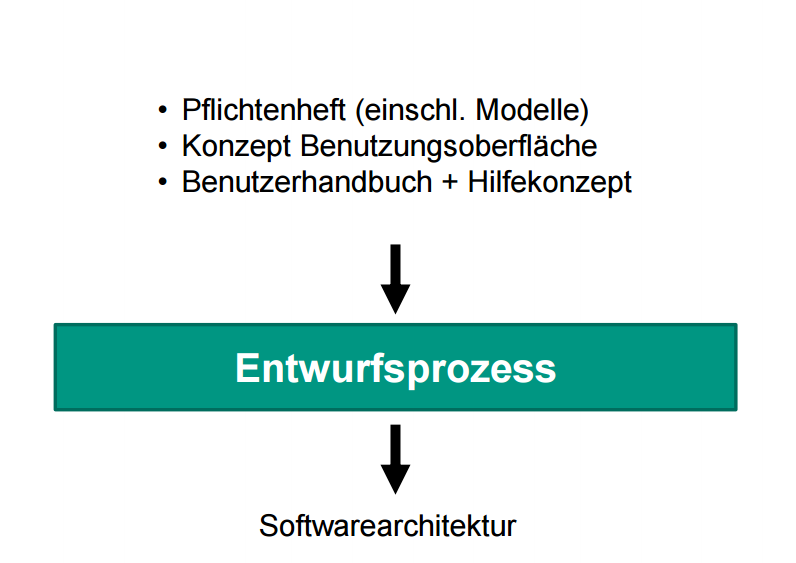
\includegraphics[scale=0.4]{./pics/tut3/design.png} \linebreak
			Softwarearchitektur ist Grundlage für Implementierung!
		\end{frame}
	
		\begin{frame}
			\frametitle{Entwurf vs Planung/Definition}
			\begin{itemize}
				\item Planung, Definition: \textbf{Was} ist zu implementieren?
				\begin{itemize}
					\item müssen wir mit dem Kunden besprechen
				\end{itemize}
				\pause
				\item Entwurf: \textbf{Wie} ist das System zu implementieren?
				\begin{itemize}
					\item können wir uns selbst überlegen
				\end{itemize}
			\end{itemize}
		\end{frame}
	
\section{Architekturstile}
	\begin{frame}{Architekturstile}
		\begin{itemize}
			\item legen den Grobaufbau der Software fest
			\begin{itemize}
				\item heißt: wir sind noch nicht (unbedingt) auf Klassen-Ebene 
			\end{itemize}
			\item in der Vorlesung besprochen
			\begin{itemize}
				\item \textbf{Schichtenarchitektur}
				\item \textbf{Klient/Dienstgeber} 
				\item \textbf{Partnernetze}
				\item \textbf{Modell-Präsentation-Steuerung}
				\item \textbf{Fließband}
				\item \textbf{Rahmenarchitektur}
				\item Datenablage
				\item Dienstorientierte Architektur
			\end{itemize}
		\end{itemize}
	\end{frame}

	\begin{frame}{Schichtenarchitektur}
	\begin{itemize}
		\item Funktionalität (Pakete, Klassen, \dots) in Schichten getrennt
		\item Schichten \enquote{aufeinander gestapelt}
		\item jede Schicht
		\begin{itemize}
			\item bietet seine Funktionalität den höheren Schichten an
			\item nutzt Funktionalität der tieferen Schichten
		\end{itemize}
		\item Arten von Schichtenarchitekturen
		\begin{itemize}
			\item intransparent: jede Schicht kann nur auf direkt darunterliegende Schicht zugreifen
			\item transparent: jede Schicht kann auch weiter unten liegende Schichten benutzen
		\end{itemize}
	\end{itemize}
	\end{frame}

\begin{frame}{Schichtenarchitektur}
	\centering 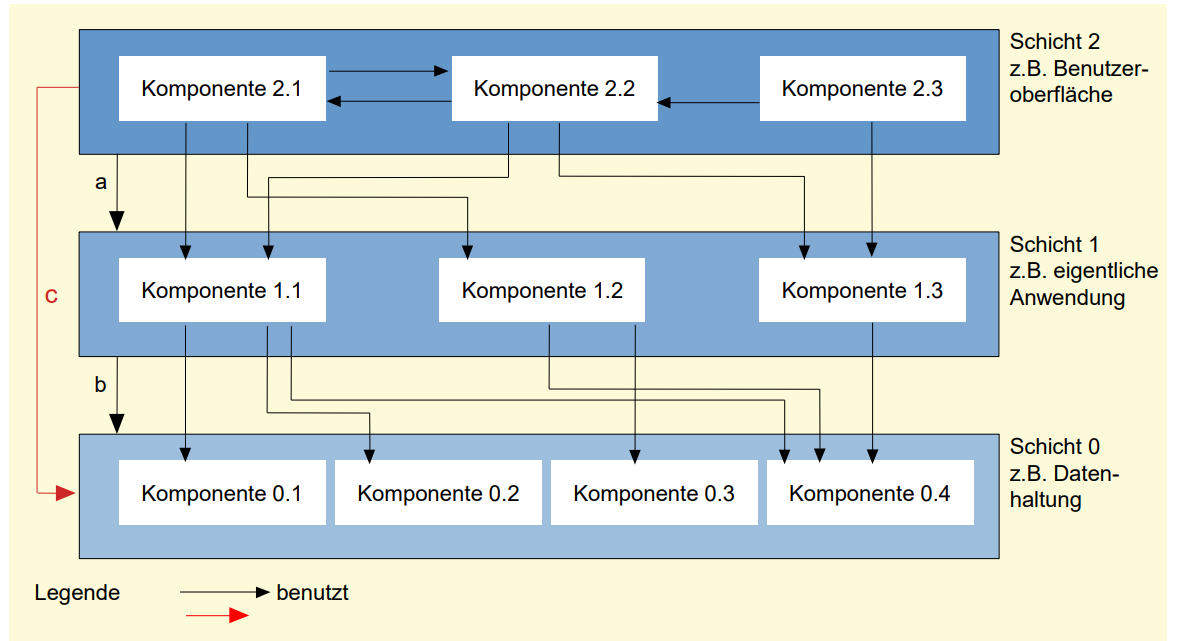
\includegraphics[scale=0.3]{pics/tut3/layers.png}
	\begin{itemize}
		\item wichtige Beispiele
		\begin{itemize}
			\item Betriebssysteme
			\begin{itemize}
				\item siehe Vorlesung \enquote{Betriebssysteme} (3. Semester)
			\end{itemize}
			\item Protokolltürme (aka. protocol stacks) 
			\begin{itemize}
				\item siehe Vorlesung \enquote{Einführung in Rechnernetze} (4. Semester)
			\end{itemize}
		\end{itemize}
	\end{itemize}
\end{frame}

\begin{frame}{Klient/Dienstgeber und Partnernetze}
	\begin{itemize}
		\item eher bekannt als \emph{Client/Server} und \emph{Peer-to-Peer}
		\item Client/Server
		\begin{itemize}
			\item Server bietet Dienst an
			\item Client nutzt diesen Dienst
		\end{itemize}
		\item Peer-to-Peer
		\begin{itemize}
			\item jeder Teilnehmer kann Dienst anbieten und nutzen
		\end{itemize}
	\end{itemize}
\end{frame}

\begin{frame}{Klient/Dienstgeber und Partnernetze}
	\centering 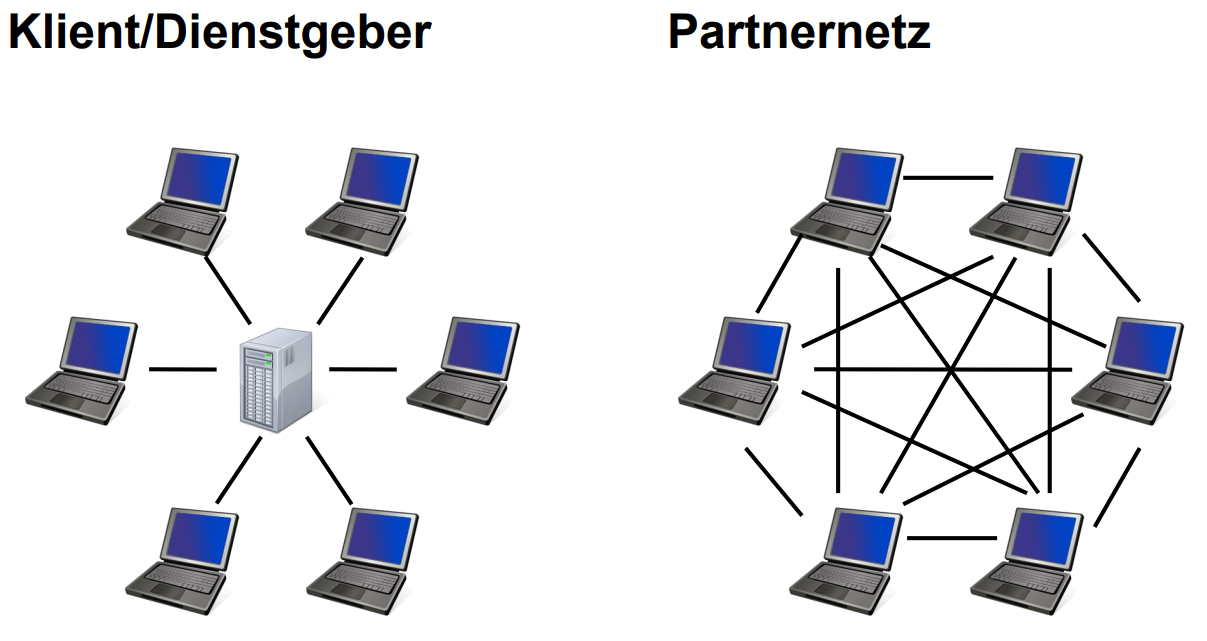
\includegraphics[scale=0.3]{pics/tut3/client-server-peer.png}
	\begin{itemize}
		\item Vor- und Nachteile jeweils?
	\end{itemize}
\end{frame}

\begin{frame}{Modell-Präsentation-Steuerung}
	\begin{itemize}
		\item eher bekannt als \emph{model-view-controller}, \emph{MVC}
		\item Software in drei große Bereiche (oft Pakete) unterteilt
		\begin{itemize}
			\item Model
			\begin{itemize}
				\item Datenspeicherung, Anwendungslogik
			\end{itemize}
			\item View
			\begin{itemize}
				\item Darstellung der Daten
				\item Schaltflächen für Benutzerinteraktion
			\end{itemize}
			\item Controller
			\begin{itemize}
				\item verwaltet Model und View
				\item zuständig für Interaktion mit Nutzer
				\item Benutzerinteraktion mit View soll Model-Daten verändern \newline $\rightarrow$ aktualisiere Model
			\end{itemize}
		\end{itemize}
	\pause
		\item Was haben wir gewonnen?
		\begin{itemize}
			\item Erweiterbarkeit: können z.B. selbes Modell verwenden für Linux, Windows, Internet
			\item Austauschbarkeit/Wartbarkeit: Model unabhängig von View
		\end{itemize}
	\end{itemize}
\end{frame}

\begin{frame}{Fließband}
	\begin{itemize}
		\item eher bekannt als \emph{pipeline}
		\item Idee: Datenverarbeitung in mehreren Stufen
		\begin{itemize}
			\item jede Stufe verarbeitet Eingabedaten zu Ausgabedaten
			\item Stufe 1 hat die Rohdaten als Eingabe
			\item jede andere Stufe hat die Ausgabe der vorherigen Stufe als Eingabe
		\end{itemize}
		\centering	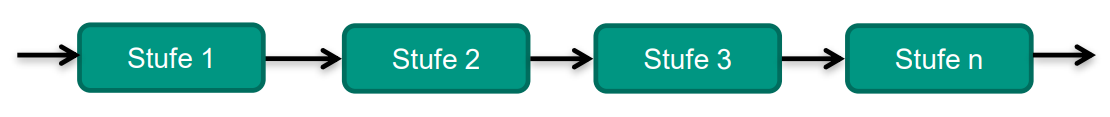
\includegraphics[scale=0.35]{pics/tut3/pipeline.png}
	\end{itemize}
		\pause
		\begin{itemize}
			\item gut anwendbar bei Verarbeitung von Datenströmen
			\item praktisch bei Parallelität: Stufen können unabhängig voneinander ausgeführt werden
		\end{itemize}
\end{frame}

\begin{frame}{Fließband bei Parallelität}
	\begin{itemize}
		\item angenommen wir haben 3-stufige Pipeline, dessen Stufen auf drei unterschiedlichen Prozessoren gleichzeitig ausgeführt werden
	\end{itemize}
	\begin{table}
		\begin{tabular}{c|c|c|c|}
				& CPU1 (Stufe 1) & CPU2 (Stufe 2) & CPU3 (Stufe 3) \\
				\hline
				t=0 & x & x & x \\
				\hline
			t=1 & Daten 1 & x & x \\
			\hline
			t=2 & Daten 2 & Daten 1 & x \\
			\hline
			t=3 & Daten 3 & Daten 2 & Daten 1 \\
			\hline
			t=4 & Daten 4 & Daten 3 & Daten 2 \\
			\hline
			t=5 & Daten 5 & Daten 4 & Daten 3 \\
			\dots & \dots & \dots & \dots 
		\end{tabular}
	\end{table}
\end{frame}

\begin{frame}{Rahmenarchitektur}
	\begin{itemize}
		\item eher bekannt als \emph{framework}
		\item Idee 
		\begin{itemize}
			\item entwickle funktionsfähiges Programm
			\item biete an bestimmten Stellen Möglichkeiten zur Erweiterung
			\begin{itemize}
				\item \emph{plug-ins}
			\end{itemize}
		\end{itemize}
		\item oft in open source Projekten verwendet
		\begin{itemize}
			\item Eclipse, Atom, VSCode, \dots
		\end{itemize}
	\end{itemize}
	\centering 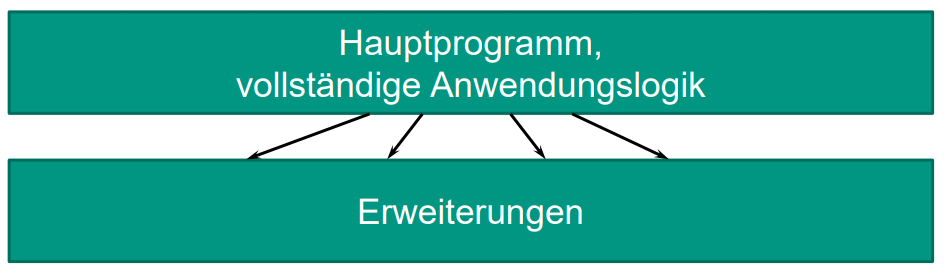
\includegraphics[scale=0.4]{pics/tut3/framework.png}
\end{frame}

\begin{frame}{Ankreuzaufgaben aus Altklausuren}
	\begin{itemize}
		\item Bei einer intransparenten Schichtenarchitektur kann eine innere Schicht nur auf direkt benachbarte Schichten zugreifen. \pause \ncorrect
		\item Schichtenarchitekturen unterstützen das Testen von Programmen. \pause \correct
		\item Ist die Benutztrelation zwischen Modulen zyklenfrei, sind Teillieferungen bei Entwicklungsverzögerungen einzelner Module möglich. \pause \correct
		\item Eine Fließband-Architektur in Software kann nur auf Parallelrechnern ausgeführt werden. \pause \ncorrect
		\item Bei einer Schichtenarchitektur mit drei übereinander liegenden Schichten kann die mittlere Schicht auf die Dienste der oberen und der unteren Schicht zugreifen. \pause \ncorrect
		\item Wenn die Benutztrelation zyklenfrei ist, heißt sie Benutzthierarchie. \pause \correct
	\end{itemize}
\end{frame}

\begin{frame}{Welcher Architekturstil ist gemeint?}
	\begin{block}{}
		\enquote{Wir wollen unseren customern solutions anbieten, die möglichst extensible sind. Falls die Software successfull ist, können wir später neuen stuff implementen, ohne den alten Code zu ändern. Über einen marketplace könnten wir dann auch noch Geld dafür getten. Sheesh.}
	\end{block}
	\pause 
	Framework
\end{frame}

\begin{frame}{Welcher Architekturstil ist gemeint?}
	\begin{block}{}
	\enquote{Auf der letzten Conference waren viele Speaker, die etwas von einer \enquote{Blockkette} erzählt haben. Da wir Amazon und Co. nicht trusten, könnten wir sowas usen um unseren Service decentralized anzubieten. Besides können wir damit money einsparen.}
	\end{block}
	\pause
	Peer-to-Peer
\end{frame}

\begin{frame}{Eine Entwurfsentscheidung :)}
	\begin{figure}
		\centering
			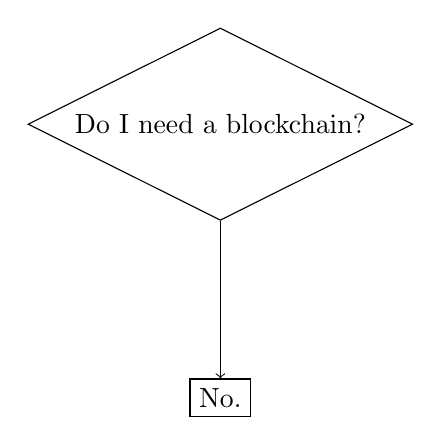
\begin{tikzpicture}
		\node [draw, diamond, aspect=2] (b) {Do I need a blockchain?};
		\node [draw, below=2cm of b] (n) {No.};
		\draw[->] (b) -- (n);
		\end{tikzpicture}
	\end{figure}

\end{frame}

\begin{frame}{Welcher Architekturstil ist gemeint?}
	\begin{block}{}
		\enquote{Ganz wichtig ist mir ja ein Separation-of-Concerns: Die Design-People sollen einen user-zentrierten Look-and-Feel entwerfen. In the meantime sollen sich die devs um neue functionality kümmern. Beide sollen independently arbeiten.}
	\end{block}
	\pause
	MVC
\end{frame}

\section{Java Swing}

\begin{frame}{Java Swing}
	\begin{itemize}
		\item mit Swing kann man GUIs bauen, ohne was anderes als Java zu benutzen
		\item graphische Elemente sind als Klassen implementiert
	\end{itemize}
	wichtige Klassen und Interfaces
	\begin{table}
		\begin{tabular}{c|l}
			\texttt{JFrame} & Fenster (nicht-blockierend) \\
			\hline
			\texttt{JDialog} & Dialogfenster (blockierend) \\
			\hline
			\texttt{JPanel} & Container, hier kommen die Bedienelemente rein\\
			\hline
			\texttt{JFileChooser} & Dateiauswahlfenster \\
			\hline
			\texttt{JButton} & Button \\
			\hline
			\texttt{JTextField} & Eingabefeld \\
			\hline
			\texttt{JMenuBar} & Menüleiste \\
			\hline
			\texttt{JLabel} & Text/Bild anzeigen \\
			\hline
			\texttt{LayoutManager} & um Layout in \texttt{JPanel} zu setzen 
		\end{tabular}
	\end{table}
\end{frame}

\begin{frame}{Übersicht}
	\centering 
	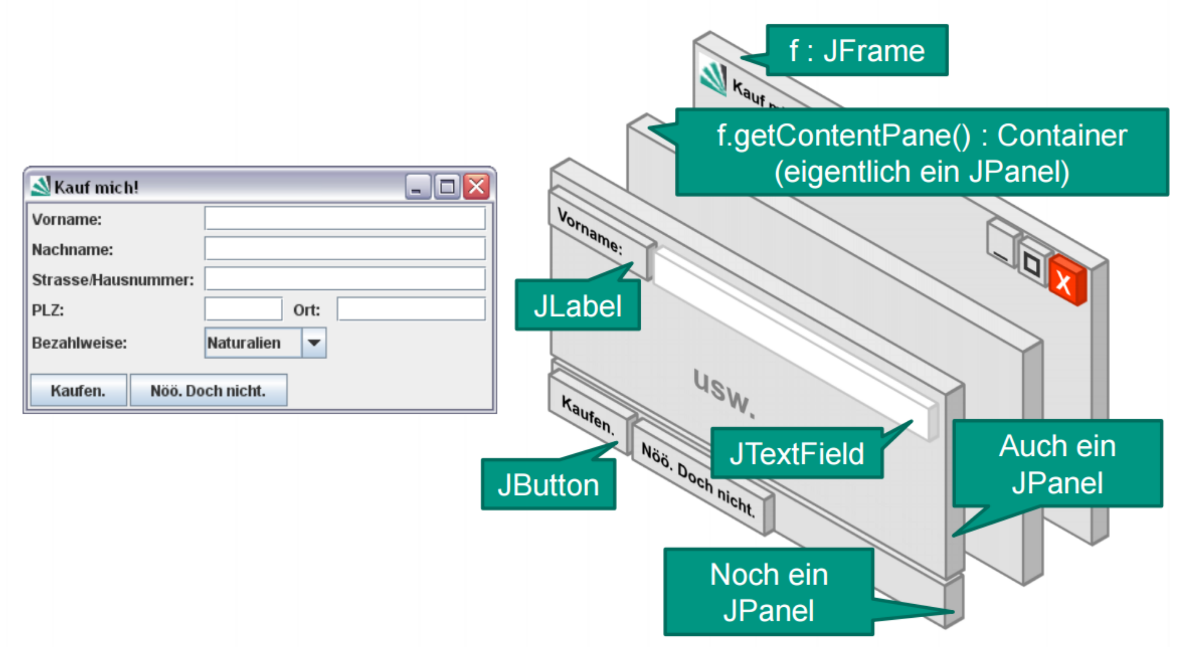
\includegraphics[scale=0.35]{pics/tut3/swing.png}
\end{frame}

\begin{frame}[fragile]{Wie erstelle ich meine eigene GUI?}
grundsätzlich 2 Möglichkeiten
\begin{block}{\texttt{JFrame} erstellen und anpassen}
	\begin{verbatim}
	JFrame f = new JFrame("Titel");
	f.add(new JButton("Knopf-Text"));
	f.setVisible(true);
	\end{verbatim}
\end{block}
\pause
\begin{block}{von \texttt{JFrame} erben, Anpassung z.B. in Konstruktor}
	\begin{verbatim}
	public class MyFrame extends JFrame { 
	    MyFrame() { add(new JButton("Knopf-Text")); // ... } 
	}
	// ...
	JFrame f = new MyFrame();
	\end{verbatim}
\end{block}
\end{frame}

\begin{frame}[fragile]{Wie erstelle ich eigene Elemente?}
	ebenfalls 2 Möglichkeiten (\texttt{JFrame} ist auch nur ein Element)
	\begin{block}{Instanzen erstellen und anpassen}
		\begin{verbatim}
			JButton b = new JButton();
			b.setText("Click me!");
			b.setToolTipText("Just do it, bro!");
		\end{verbatim}
	\end{block}
	\pause
		\begin{block}{Klassen überschreiben, Anpassung z.B. in Konstruktor}
		\begin{verbatim}
public class MyButton extends J7Button { 
    MyButton() { setText("Click me!"); // ... } 
}
		// ...
		JButton b = new MyButton();
		\end{verbatim}
	\end{block}
\end{frame}


\begin{frame}{Link-Sammlung}
	\begin{itemize}
		\item allgemeine Anlaufstelle
		\begin{itemize}
			\item \url{https://docs.oracle.com/javase/tutorial/uiswing/}
		\end{itemize}
		\item Layout Manager erklärt
		\begin{itemize}
			\item \url{https://docs.oracle.com/javase/tutorial/uiswing/layout/visual.html}
		\end{itemize}
		\item jedes Element erklärt
		\begin{itemize}
			\item \url{https://docs.oracle.com/javase/tutorial/uiswing/components/componentlist.html}
		\end{itemize}
	\end{itemize}	
\end{frame}

\begin{frame}{Praxis-Zeit}
	\huge \centering kleines Beispiel
\end{frame}

\section{Entwurfsmuster}
	\subsection{Grundlagen}
	\begin{frame}
		\frametitle{Empfehlenswerte Literatur (wirklich!)}
		\begin{itemize}
			\item knapp 700 Seiten
			\begin{itemize}
				\item als interaktives Nachschlagewerk
			\end{itemize}
		\end{itemize}
		\centering
		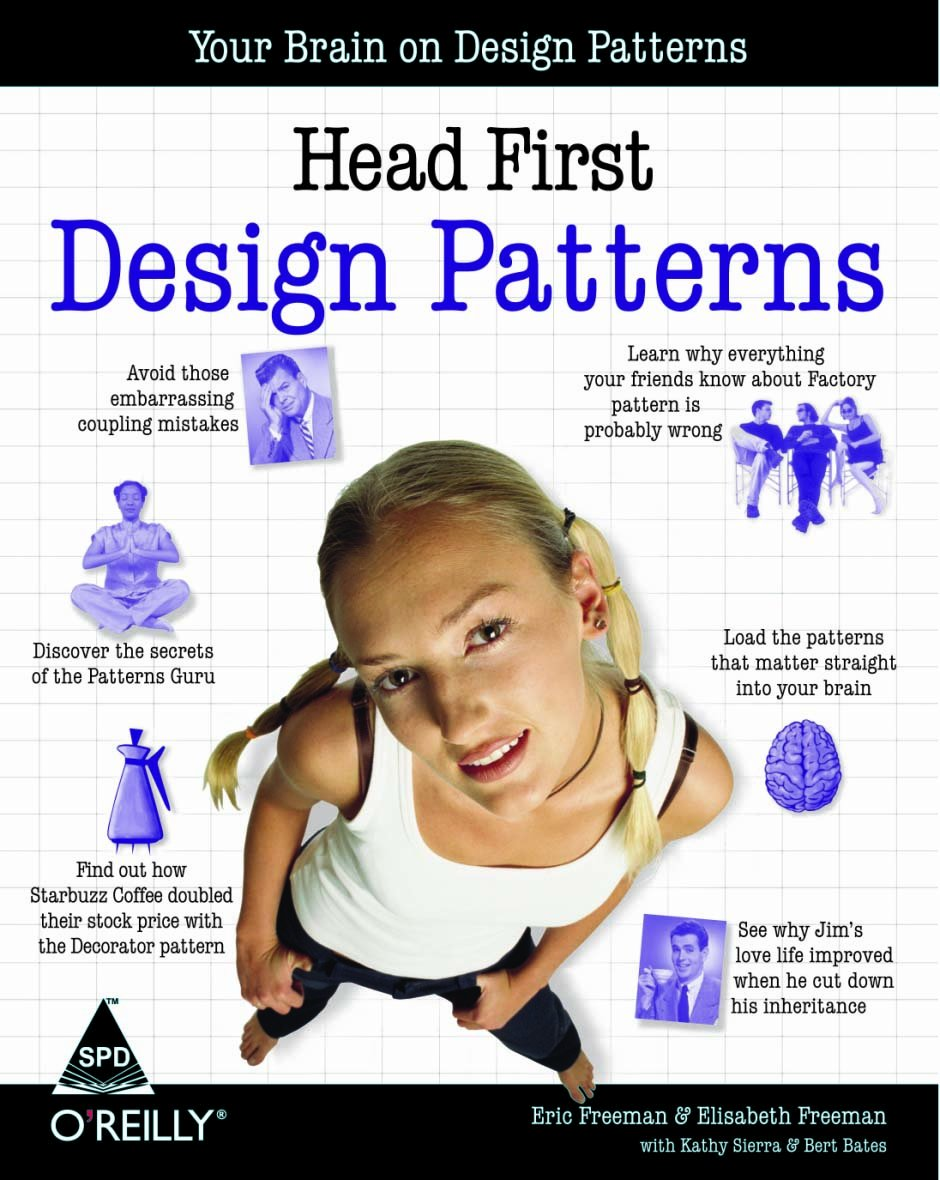
\includegraphics[scale=0.15]{./pics/tut3/literature.jpg}
	\end{frame}
		
	\begin{frame}
		\frametitle{Was sind Entwurfsmuster?}
		\begin{block}{Entwurfsmuster}
			Ein Software-Entwurfsmuster beschreibt eine
			Familie von Lösungen für ein Software-Entwurfsproblem.
		\end{block}
		\pause
		\begin{itemize}
			\item schematische Klassendiagramme zur Lösung von häufig auftretenden Problemen \pause
			\item Wiederverwendung von Entwurfswissen $\implies$ Rad nicht neu erfinden!
		\end{itemize}
		\pause
		\centering
		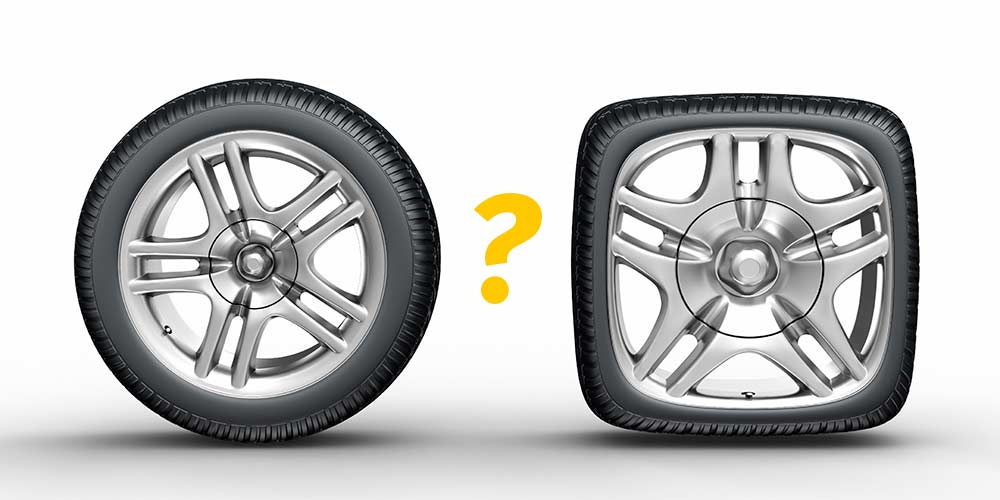
\includegraphics[scale=0.2]{./pics/tut3/new-wheel.jpg}
	\end{frame}

	\begin{frame}
		\frametitle{Wozu Entwurfsmuster?}
		\begin{itemize}
			\item erleichtern Kommunikation \pause
			\item erleichtern "'gute"' Entwürfe 
			\begin{itemize}
				\item damit auch das Schreiben von wartbarem/erweiterbarem Code
			\end{itemize}
		\end{itemize}
\end{frame}
	
	\begin{frame}
		\frametitle{Geheimnisprinzip}
		\begin{block}{Geheimnis- / 
				Kapselungsprinzip}
			Jedes Modul verbirgt eine wichtige
			Entwurfsentscheidung hinter einer
			wohldefinierten Schnittstelle, die sich bei einer
			Änderung der Entscheidung nicht mit ändert.
		\end{block}
		\pause
		\begin{alertblock}{Warum eigentlich? Lokalitätsprinzip!}
			lokale Änderungen sollen sich nicht auf andere Teile auswirken 
			\linebreak $\implies$ weniger Fehler und Arbeit
		\end{alertblock}
		Beispiel? \pause $\implies$ private Attribute mit get()- und set()-Methoden
	\end{frame}

	\begin{frame}
		\frametitle{Vorgriff: Entwurfsmuster Strategie}
		\begin{itemize}
			\item Ziel: Algorithmen kapseln, austauschbar machen
			\item wird in vielen Entwurfsmustern verwendet
		\end{itemize}
		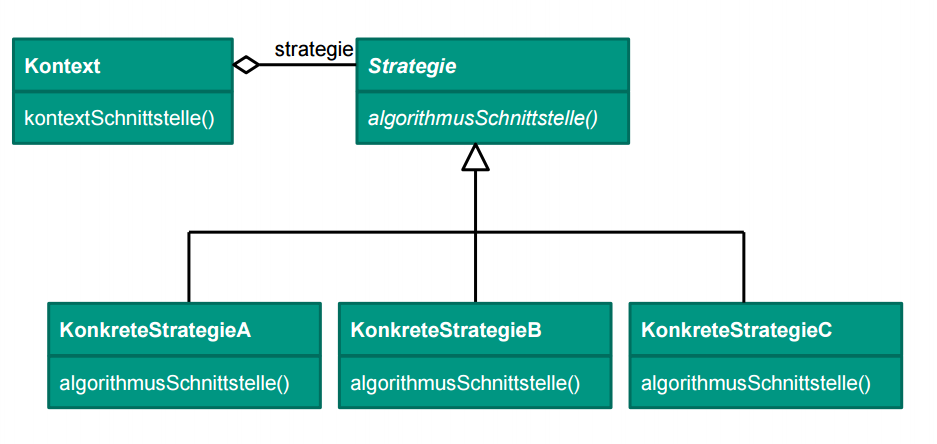
\includegraphics[scale=0.5]{./pics/tut3/strat.png}
	\end{frame}

	\begin{frame}
		\frametitle{Quiz (Ankreuzaufgaben aus Klausuren)}
		Wahr oder falsch?
		\begin{itemize}
			\item Das Entwurfsmuster Strategie bietet die Möglichkeit, eine Klasse mit einer von mehreren möglichen Verhaltensweisen zu konfigurieren. \pause \textcolor{green}{\cmark} \pause
			\item Das Muster Strategie kapselt austauschbares Verhalten und verwendet Delegierung, um zu entscheiden, welches Verhalten verwendet wird. \pause \textcolor{green}{\cmark} \pause 
			\item Das Hinzufügen einer neuen konkreten Strategie erfordert keine Änderung existierender konkreter Strategien. \pause \textcolor{green}{\cmark}
		\end{itemize}
\end{frame}

	\begin{frame}
		\frametitle{Kategorien der Entwurfsmuster}
		\begin{itemize}
			\item \textbf{Entkopplungs-Muster}
				\begin{itemize}
					\item \textbf{Adapter}
					\item \textbf{Beobachter}
					\item \textbf{Iterator}
					\item \textbf{Stellvertreter}
					\item \textbf{Vermittler}
					\item Brücke
				\end{itemize}
			\item Varianten-Muster
			\item Zustandshandhabungs-Muster
			\item Steuerungs-Muster
			\item Bequemlichkeits-Muster
		\end{itemize}
	\end{frame}

	\begin{frame}
		\frametitle{Entkopplungs-Muster}
		\begin{itemize}
			\item übergeordnetes Ziel: System in Teile aufspalten, die unabhängig voneinander sind
			\linebreak $\implies$ Teile austauschbar bzw. veränderbar
	\end{itemize}
	\end{frame}

	\subsection{Adapter}
	\begin{frame}
		\frametitle{Adapter}
		\begin{block}{Problem}
			\begin{itemize}
				\item Klassen mit inkompatiblen Schnittstellen, die wir aber zusammen benutzen wollen 
				\item Schnittstellen nicht änderbar (z.B. externe Bibliotheken)
			\end{itemize}
		\end{block}
		\pause
		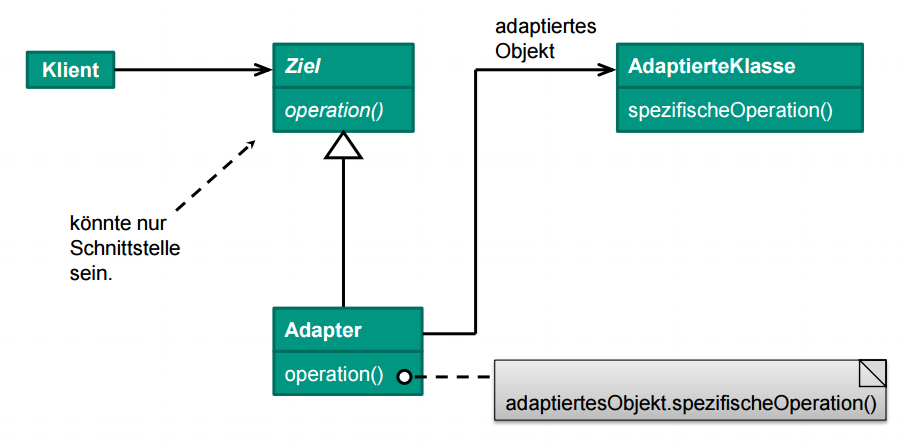
\includegraphics[scale=0.45]{./pics/tut3/adap-obj.png}
	\end{frame}

	\begin{frame}
		\frametitle{Adapter (Objektadapter)}
		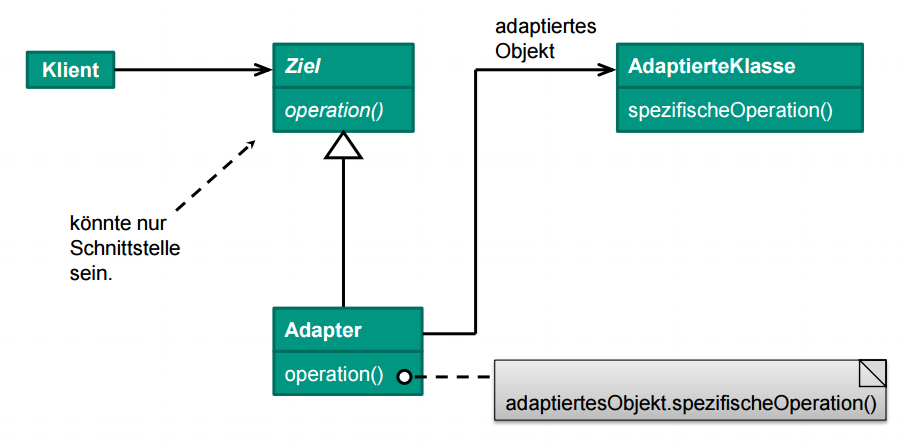
\includegraphics[scale=0.45]{./pics/tut3/adap-obj.png}
		\begin{block}{Wir sind bei Entkopplung-Mustern, Preisfrage:}
			Wo ist hier die Entkopplung?
			\pause
			\linebreak der Klient ist von der adaptierten Klasse entkoppelt $\implies$ austauschbar
		\end{block}
	\end{frame}

	\begin{frame}
		\frametitle{Adapter - Alternative (Klassenadapter)}
		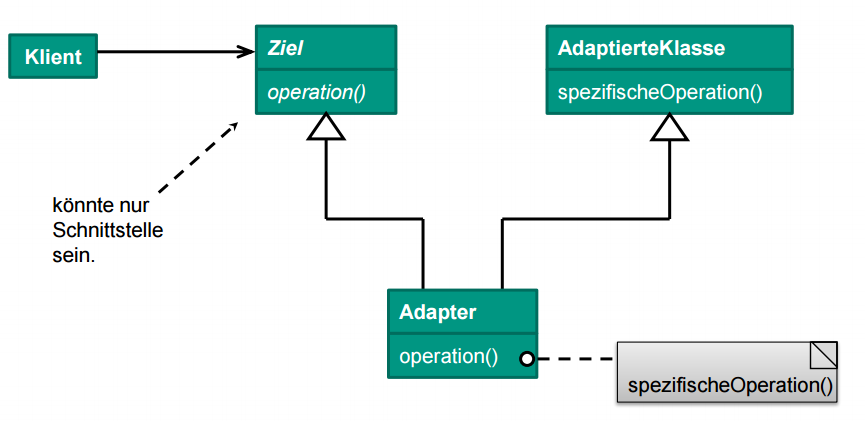
\includegraphics[scale=0.45]{./pics/tut3/adap-cl.png} \linebreak \pause
		Was für ein Problem bekommt ihr, wenn ihr das auf einem ÜB implementieren müsst? \pause \linebreak
		$\implies$ keine Mehrfachvererbung in Java!
	\end{frame}

	\subsection{Beobachter}
	\begin{frame}{Beobachter/Observer: abstrakt}
		\begin{block}{Problem}
			\begin{itemize}
				\item ein Subjekt, viele Beobachter
				\item Subjekt ändert Zustand $\implies$ Beobachter machen "'irgendwas"
			\end{itemize}		
		\end{block}
	\end{frame}

	\begin{frame}{}
		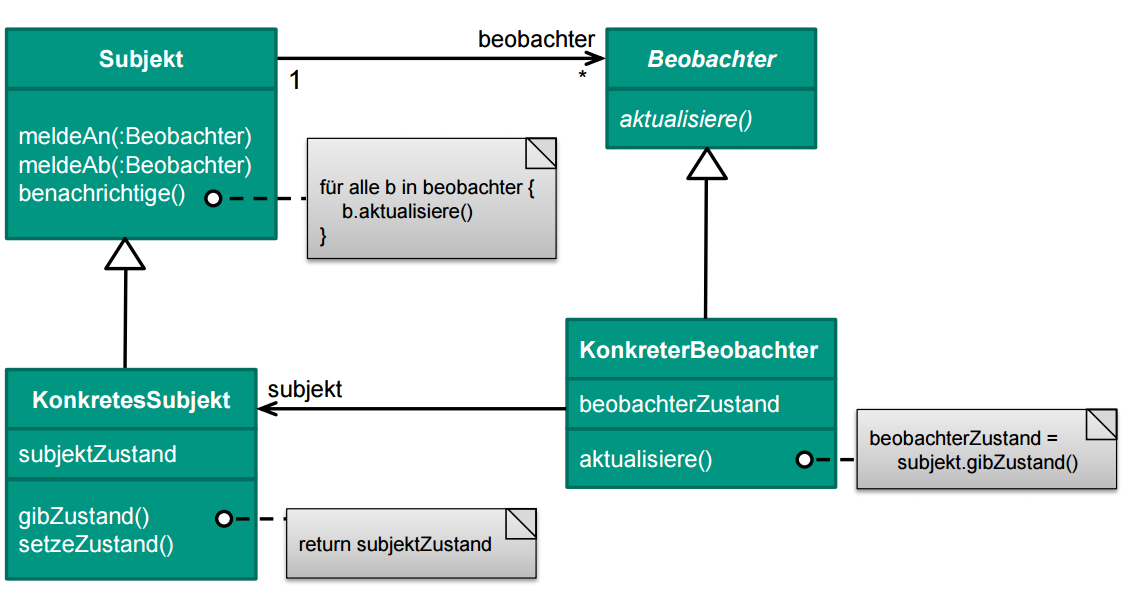
\includegraphics[keepaspectratio, width=\textwidth, height=\textheight]{pics/tut3/obs.png}
		\pause
		\begin{block}{Entkopplung?}
		\begin{itemize}
			\pause 
			\item jeder Beobachter definiert, was bei Benachrichtigung passiert, Subjekt kriegt davon nichts mit \pause
			\item zur Laufzeit änderbar: Anzahl der Beobachter
		\end{itemize}
		\end{block}
	\end{frame}

	\begin{frame}{Beobachter/Observer: am Beispiel}
		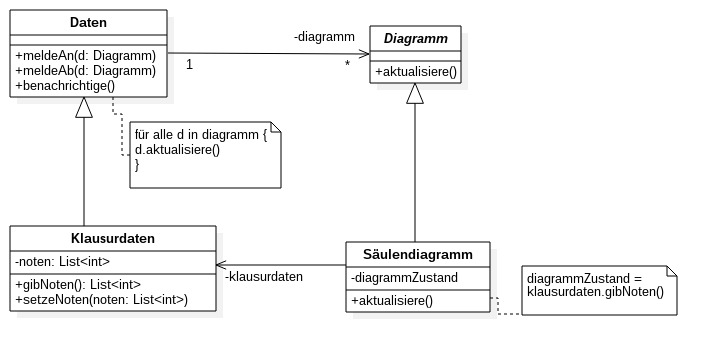
\includegraphics[keepaspectratio, width=\textwidth, height=\textheight]{pics/tut3/observer_example.jpg}
	\end{frame}

\begin{frame}[fragile]{Beobachter=Listener in Java Swing}
	\centering
	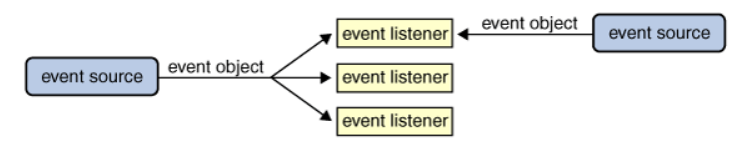
\includegraphics[scale=0.5]{pics/tut3/listener.png}
	\pause
	\begin{block}{Beobachter für einen \texttt{JButton btn}}
		\begin{verbatim}
			btn.addActionListener(new ActionListener() {
			    @Override
			    public void actionPerformed(ActionEvent e) {
			        System.out.print("clicked");
			    }
			});
		\end{verbatim}
	\end{block}
\end{frame}

\begin{frame}[fragile]{Beobachter=Listener in Java Swing}
	\centering
	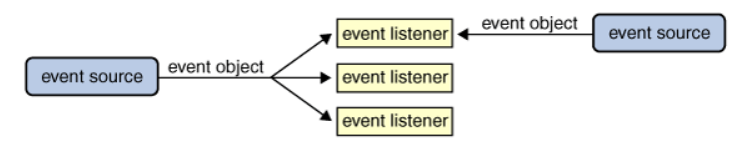
\includegraphics[scale=0.5]{pics/tut3/listener.png}
	\begin{block}{Das Gleiche mit Lambdas}
		\begin{verbatim}
		btn.addActionListener(e -> System.out.print("clicked"));
		\end{verbatim}
	\end{block}
\end{frame}

	\subsection{Iterator}
	\begin{frame}
		\frametitle{Iterator}
		\begin{block}{Problem}
			\begin{itemize}
				\item wollen über Datenstruktur iterieren + Operationen ausführen \pause
				\item das Ganze ohne Kentniss des internen Aufbaus der Datenstruktur 
			\end{itemize}
		\end{block}
		\pause
		\centering
		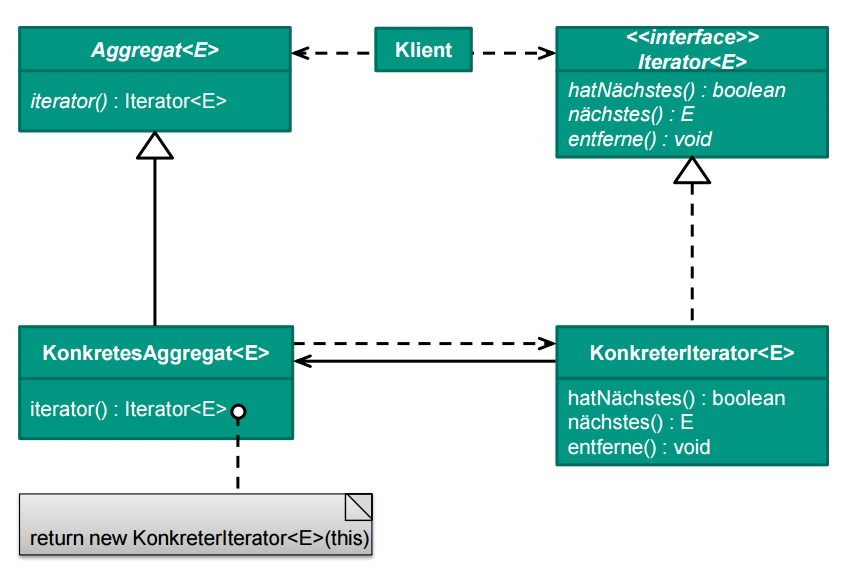
\includegraphics[scale=0.35]{./pics/tut3/iter.png}
	\end{frame}

	\begin{frame}
		\frametitle{Iterator}
		\centering
		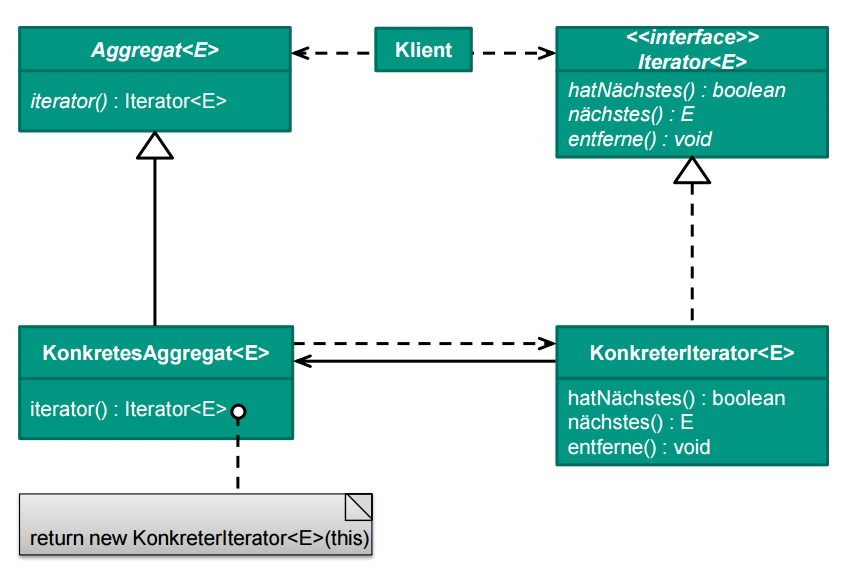
\includegraphics[scale=0.35]{./pics/tut3/iter.png}
		\begin{block}{Entkopplung?}
			\begin{itemize}
				\pause 
				\item Klient benutzt nur Methoden der Schnittstelle auf dem konkreten Iterator \linebreak $\implies$ Implementierung austauschbar
			\end{itemize}
		\end{block}
	\end{frame}
	
	\begin{frame}
		\frametitle{Iterator}
		\centering
		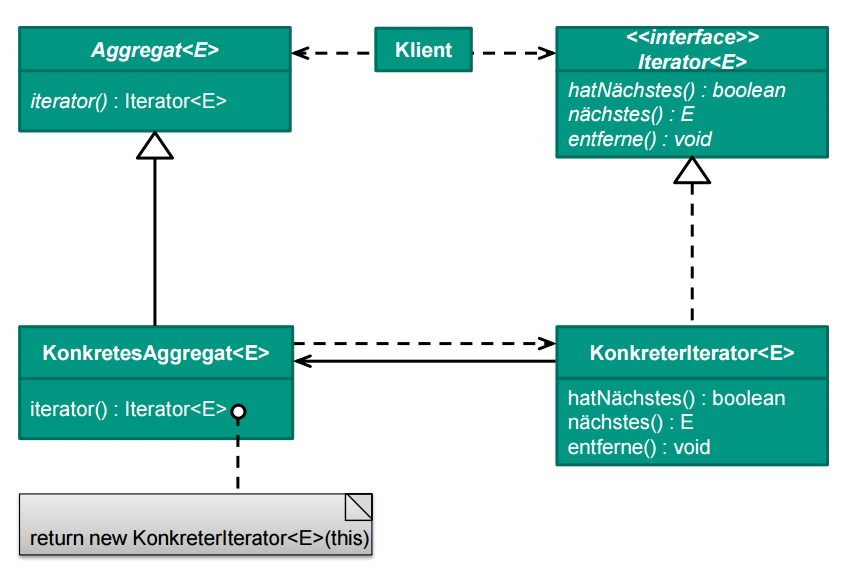
\includegraphics[scale=0.35]{./pics/tut3/iter.png}
		\linebreak Beispiel in Java: \texttt{list.iterator()};
	\end{frame}

	\begin{frame}
		\frametitle{Quiz (Ankreuzaufgaben aus Klausuren)}
		Wahr oder falsch?
		\begin{itemize}
			\item Klienten können mithilfe des Iterator-Musters Sammlungen von Objekten und einzelne Objekte auf die gleiche Weise behandeln. \pause \ncorrect \pause
			\item Das Entwurfsmuster Iterator ist den Variantenmustern zuzuordnen. \pause \ncorrect
		\end{itemize}
	\end{frame}

	\subsection{Stellvertreter}
	\begin{frame}
		\frametitle{Stellvertreter}
		\begin{block}{Problem}
			\begin{itemize}
				\item wollen Zugriff auf ein Objekt kontrollieren, ohne seine Klasse zu ändern \linebreak \pause $\implies$ Stellvertreter macht Zugriffskontrolle
			\end{itemize}
		\end{block}
		\pause
		\centering
		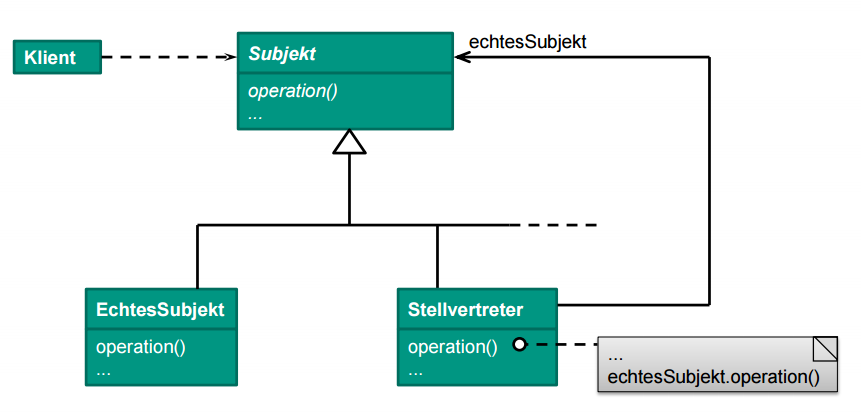
\includegraphics[scale=0.4]{./pics/tut3/prox.png}
	\end{frame}

	\begin{frame}
		\frametitle{Stellvertreter}
		\centering
		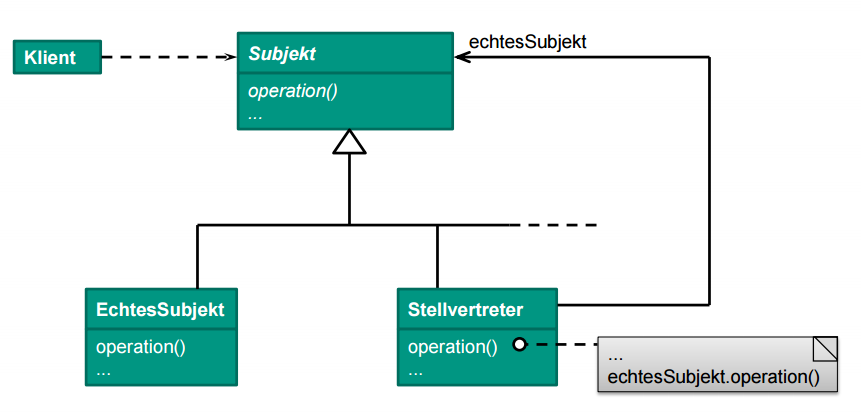
\includegraphics[scale=0.4]{./pics/tut3/prox.png}
		\begin{block}{Entkopplung?}
			\begin{itemize}
				\pause 
				\item Klient hat keinen direkten Zugriff auf das echte Subjekt
			\end{itemize}
		\end{block}
	\end{frame}

%TODO proxy vs adapter?

	\subsection{Vermittler}
		\begin{frame}
		\frametitle{Vermittler}
		\begin{block}{Problem}
			\begin{itemize}
				\item mehrere voneinander abhängige Objekte \linebreak \pause $\implies$ Zustände der Objekte von anderen Zuständen abhängig
			\end{itemize}
		\end{block}
		\pause
		\centering
		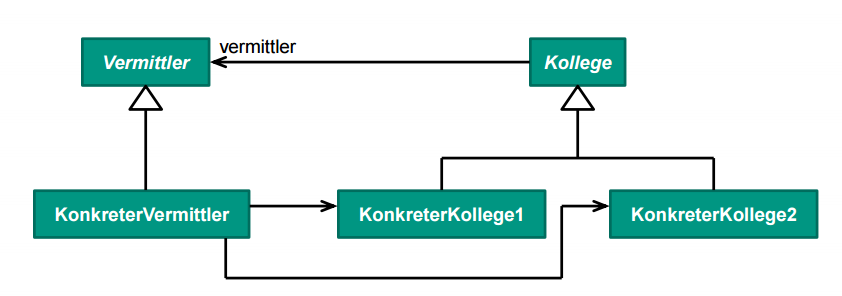
\includegraphics[scale=0.45]{./pics/tut3/med.png}
	\end{frame}

	\begin{frame}
		\frametitle{Vermittler}
		\centering
		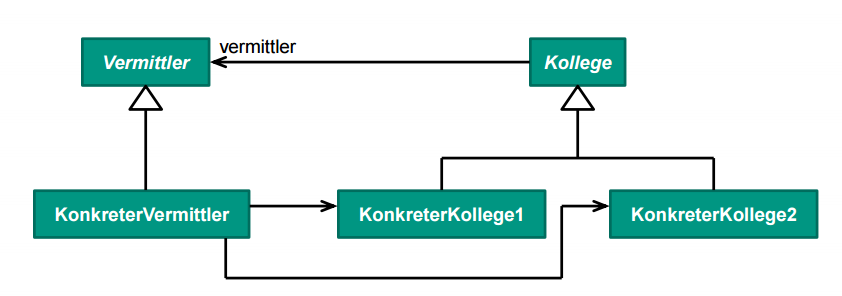
\includegraphics[scale=0.45]{./pics/tut3/med.png}
		\begin{block}{Entkopplung?}
			\begin{itemize}
				\pause 
				\item Kollegen kennen sich nicht direkt  \linebreak \pause $\implies$ Hinzufügen eines Kollegen erfordert keine Änderung der alten Kollegen
			\end{itemize}
		\end{block}
	\end{frame}

	\subsection{Aufgabe}
	\begin{frame}
		\frametitle{Klausuraufgabe (Hauptklausur SS 2012)}
		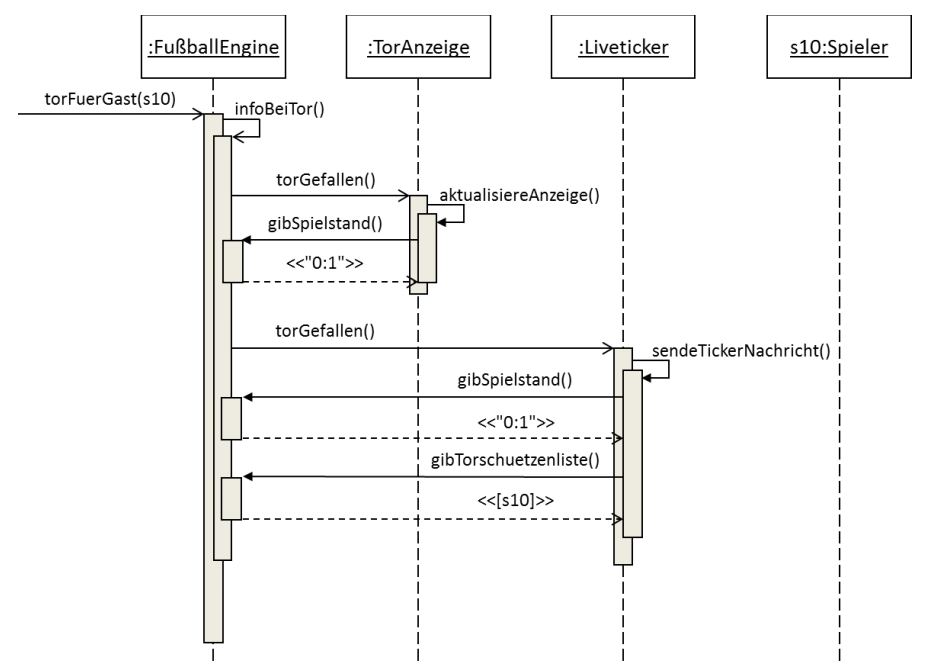
\includegraphics[scale=0.35]{./pics/tut3/obs-task.png}	
		\begin{block}{Aufgabe 1}
			Welches Entwurfsmuster erkennen Sie in diesem Diagramm? \pause
			Beobachter.
		\end{block}
	\end{frame}

	\begin{frame}
			\begin{small}
				Entwerfen Sie das folgende Klassendiagramm passend zu dem Sequenzdiagramm; es soll
				alle verwendeten Klassen und Methoden enthalten. Kennzeichnen Sie die Zugreifbarkeiten
				der Methoden mit den Symbolen +, -, \#; seien Sie dabei möglichst restriktiv. Verzichten
				Sie auf die Modellierung von Attributen. Kennzeichnen Sie die Elemente
				des Entwurfsmusters und deren Funktion.
			\end{small}
			\linebreak
			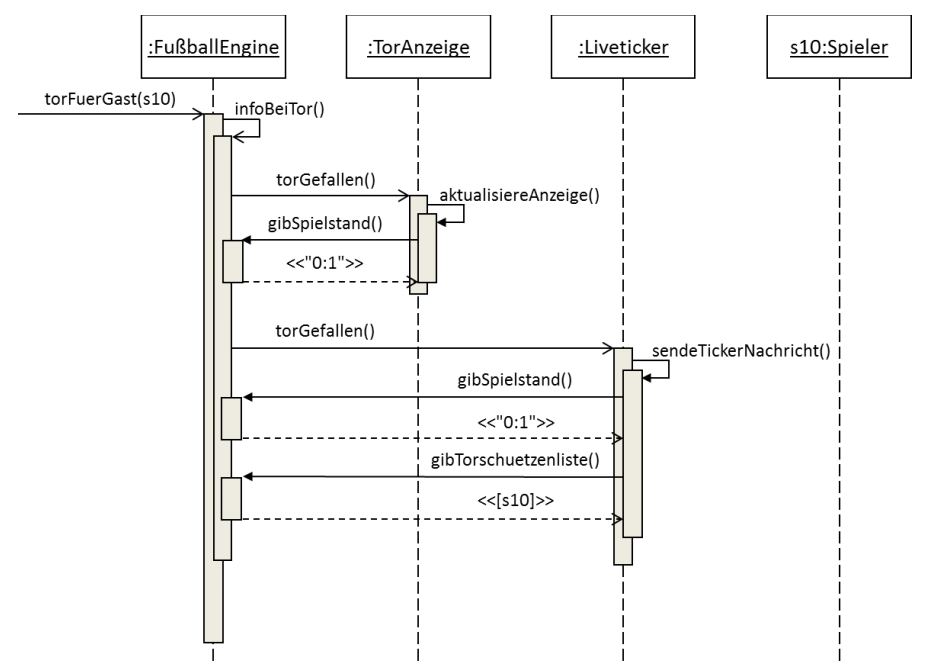
\includegraphics[scale=0.35]{./pics/tut3/obs-task.png}
	\end{frame}

	\begin{frame}
		\frametitle{Musterlösung}
		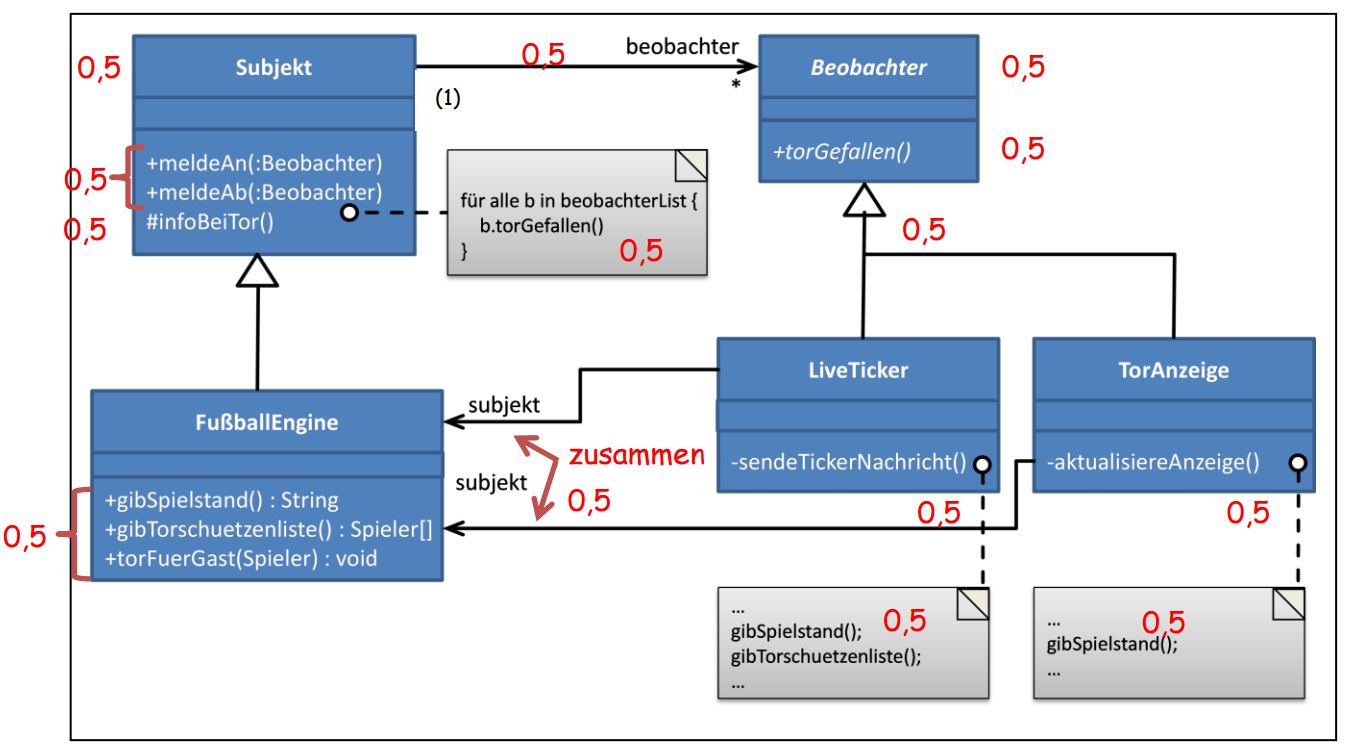
\includegraphics[scale=0.35]{./pics/tut3/obs-task-sol.png}
	\end{frame}
	
\section{Ende}	
	\begin{frame}
		\frametitle{Bis dann! (dann  := 25.06.19)}
		\centering
		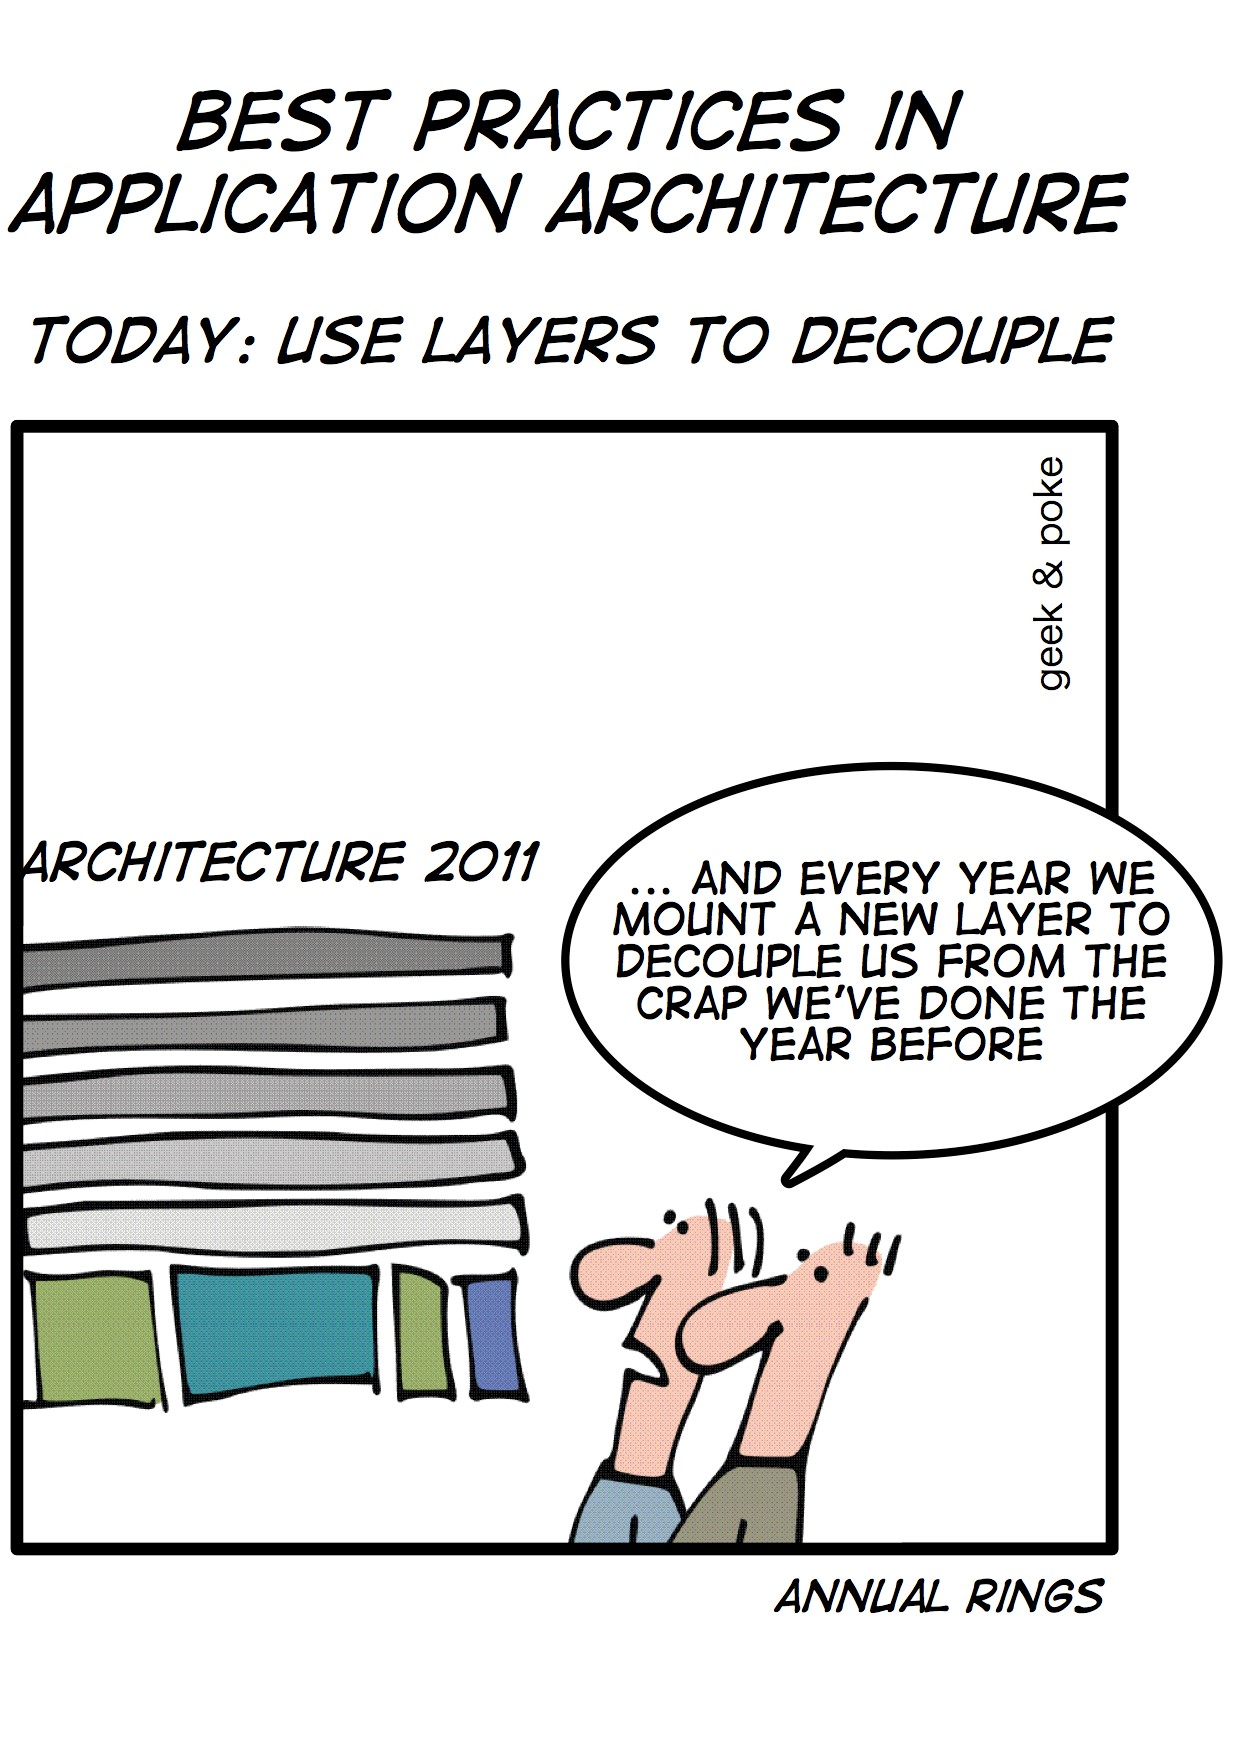
\includegraphics[scale=0.55]{./comics/footprints2.jpg}
	\end{frame}

\end{document}